\documentclass[conference]{IEEEtran}
\IEEEoverridecommandlockouts
% The preceding line is only needed to identify funding in the first footnote. If that is unneeded, please comment it out.
\usepackage{amsmath,amssymb,amsfonts}
\usepackage{algorithmic}
\usepackage{graphicx}
\usepackage{textcomp}
\usepackage{xcolor}
\usepackage[backend=biber, style=ieee,]{biblatex}
\addbibresource{citations.bib}
\graphicspath{{images/}}
\begin{document}

\title{Wireless Mesh Networks and their Applications}

\author{\IEEEauthorblockN{Colter Roche}
\IEEEauthorblockA{\textit{Computer Science} \\
\textit{Florida Polytechnic University}\\
croche2574@floridapoly.edu}
}

\maketitle

\begin{abstract}
This report aims to provide a general overview of mesh networks, their uses, and different aspects of development and implementation.
\end{abstract}
\section{Introduction}
Wireless mesh networks are a decentralized network of individual devices capable of sending, receiving and transferring data to other devices on the network, with a mesh topology.
Mesh networks can be fully connected, with every node linked to every other node directly, or more commonly, partially linked. There are no central
servers or infrastructure for linking and routing, and individual nodes can be added or removed with minimal disruption\cite{ramanathan_2018}.  Mesh networks are frequently used for military and emergency
response networks, given their flexibility and need for connectivity in remote areas.  More recently, mesh networks have also found practical use for IoT device connections and providing
WiFi coverage to larger areas.  

Mesh networks have two main methods of sending data, flooding or routing.  Flooding sends packets to every outgoing link on the network, ensuring the data reaches
its destination, but uses a larger amount of bandwidth sending unneeded data to every device.  Routing avoids this waste by sending packets to specific nodes in the network along specific paths.  
Special algorithms are required to account for nodes dropping in and out of the network\cite{enwiki:1003045519}.  
\section{History and Development}
The origins of mesh networks lie with the military and emergency response situations.  One of the first networks was the ALOHA packet radio network in Hawaii, used to connect the islands.
The challenges of controlling access to communication channels with multiple nodes connected at the same time led to the eventual creation of packet radio communications protocols and inspired the 
creation of Ethernet LAN network systems.  DARPA expanded on these topics in the early 1970's as a way to replicate ARPANET, an internet precursor, in a wireless context.
\begin{figure}[htbp]
    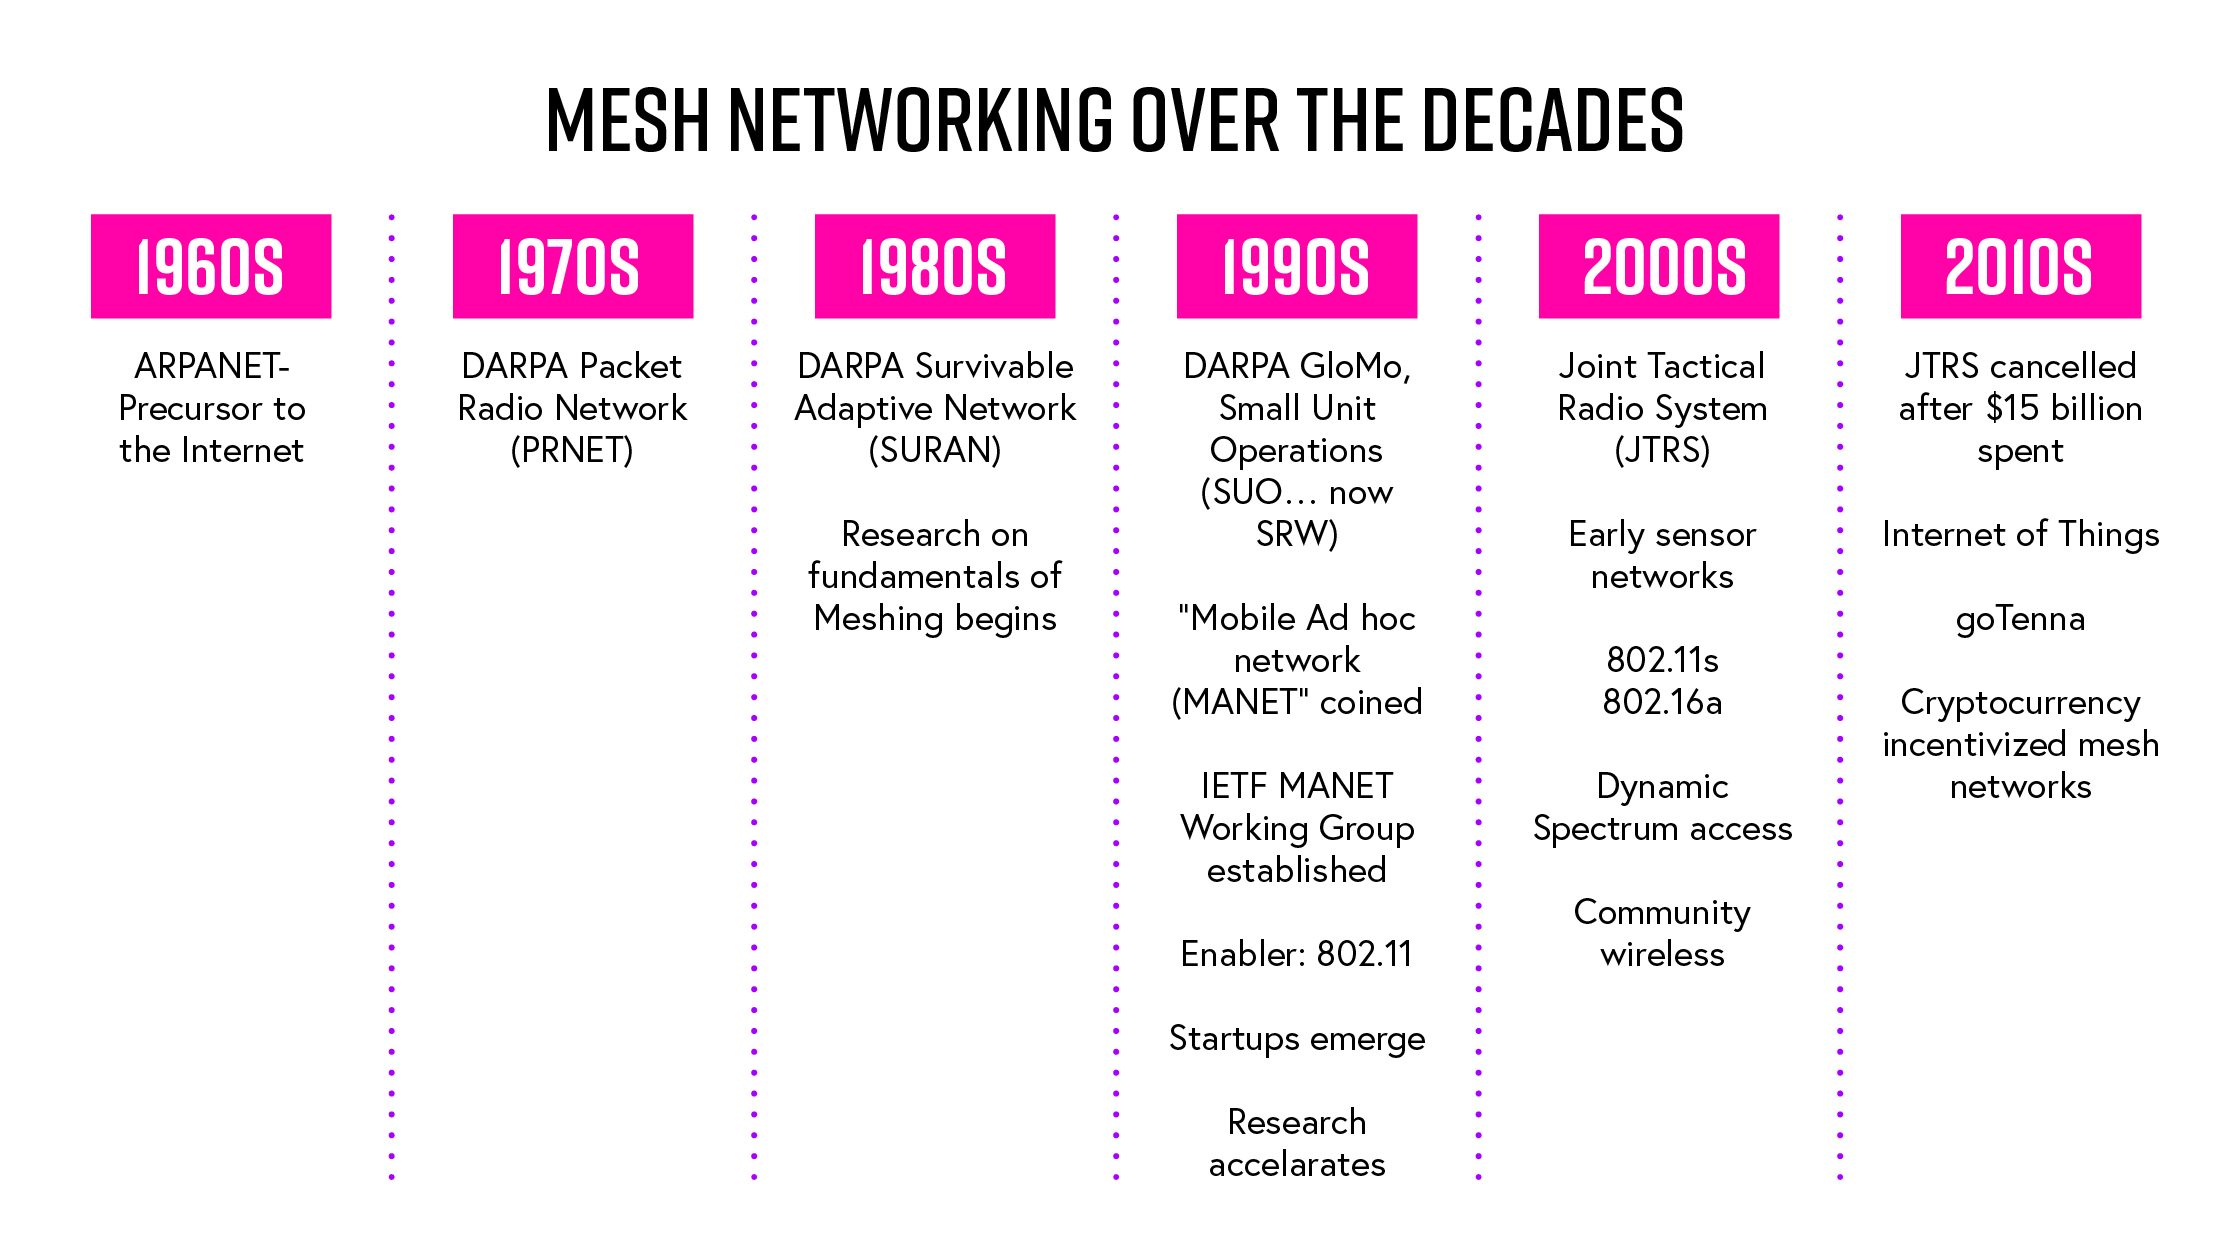
\includegraphics[width=0.5\textwidth]{timeline.jpg}
    \caption{Timeline of mesh network development \cite{ramanathan_2018}}
\end{figure}

In the 90's, Mobile Ad hoc Networks (MANET) were developed, consisting of a routable network environment on top of an ad hoc link layer network. In a MANET environment, there aren't any fixed location nodes
or stationary infrastructure\cite{geeksforgeeks_2020}.  Individual nodes serve as router and access points.  Since there are no nodes guaranteed to be available, maintaining the information required to route connections is more difficult.
Bandwidth and throughput are also reduced even compared to radio based networks.  MANET is used primarily for emergency services, military applications, and sensor networks.  Wireless Mesh Networks are very similar 
to MANET, except non-mobile routers and mesh nodes are allowed.  Data is sent across multiple frequencies as well, allowing for higher throughput and more bandwidth.  By passing packets from node to node, networks  
are able to stretch over larger areas while still maintaining reasonably high speeds compared to wired networks.
\section{Comparison of Protocols} 
There are four major types of routing protocols for ad hoc and mesh networks:
\begin{itemize}
    \item Table Driven Routing
    \item On Demand Routing
    \item Hybrid Routing
    \item Hierarchical Routing
\end{itemize}
Each protocol type has advantages and disadvantages for routing packets.  Examples of each type, as well as some other important protocols, are described in more detail below.
\subsection{OLSR and B.A.T.M.A.N.}
The Optimized Link State Routing Protocol (OLSR) is a table-driven protocol that exchanges routing data with other nodes in the network proactively.  Rather than flooding the
entire network to establish routing info, certain nodes are designated as Multipoint Relays (MPRs), and then the MPRs handle routing and distribution to the rest of the network.
MPRs are linked to nodes with bidirectional links, avoiding issues with acknowledgements not getting returned correctly, and routing info is periodically distributed to the rest 
of the network as part of the MPR control messages\cite{clausen_jacquet_2003}.  Some advantages of OLSR are less end-to-end delay and less control message issues even when the links are unreliable, due to the 
periodic sending of messages by MPR nodes. Discovery and re-linking broken links takes a large amount of time, however, and there is more overhead to keep track of mobile nodes and the 
routing table\cite{researchgate}.

The Better Approach To Mobile Ad hoc Networking (B.A.T.M.A.N.) aims to fix some of the issues faced with OLSR implementations.  Instead of multiple nodes needing to store information about 
the network and distribute that info to the rest of the network periodically, individual nodes save information about the direction they received the data from, and then pass that information on
to the rest of the network\cite{why-starting-batman}. B.A.T.M.A.N. implements routing on the lower link level, directly handling the packet transmission, while OLSR is implemented in the network layer.  Nodes still broadcast there location to 
the network, but only to the nodes directly adjacent. Those nodes then forward that info to adjacent nodes, and this covers the whole network.  When a packet is sent, the directional information of each node is used to 
dynamically find the shortest path. This lack of overhead makes B.A.T.M.A.N. significantly faster than OLSR when dealing with broken links.  
\subsection{ABR and DSR}
Associativity Based Routing (ABR) is a three stage, on demand routing protocol with low overhead and no use of routing tables.  Instead of maintaining routes for all possible transmission routes, only the routes 
currently needed are stored.  Routes that are no longer needed are deleted, and if a link is broken, a new path is generated from the last functional node\cite{toh_1997}. 

To generate a path, the route discovery phase sends a search packet to find the destination node. Once that node is found, the destination node sends a reply packet back along the shortest path found, finalizing that path 
in the routing table of any nodes along the path.  If a link breaks due to a node disconnect or other issue, the last functioning upstream node is able to perform the route discovery phase on a smaller scale to reconnect the 
route.  Once the route is no longer needed or has grown stale, the path information is deleted.  This greatly reduces the overhead and required computational power such a network requires, allowing for lower power implementations.

Dynamic Source Routing (DSR) is similar to ABR in that paths are discovered dynamically, but unlike ABR, path information for all previous nodes is cached at each node along the path during discovery.  In the case of a lost node, the records 
of that node need to be purged from all routing tables and node discovery will need to run again\cite{johnson_2007}.  Unfortunately, there can be significant overhead and delay during the route discovery phase, especially in large networks with many mobile nodes.
\subsection{ZRP}
The Zone Routing Protocol (ZRP) is a hybrid routing protocol implementing proactive and reactive routing. Mesh networks are divided into overlapping zones containing all nodes within a certain radius. Nodes within the routing zone keep a routing
table for tracking paths, and a route discovery protocol is used to find the paths between routing zones. Nodes are only required to track the network links locally within zones, and updates are also handled locally.  Verifying whether a particular
zone contains the destination node only requires a quick lookup against the local routing table\cite{haas}.  This allows for much larger networks with lower overhead than previously discussed table and path-based protocols.  
\begin{figure}[htbp]
    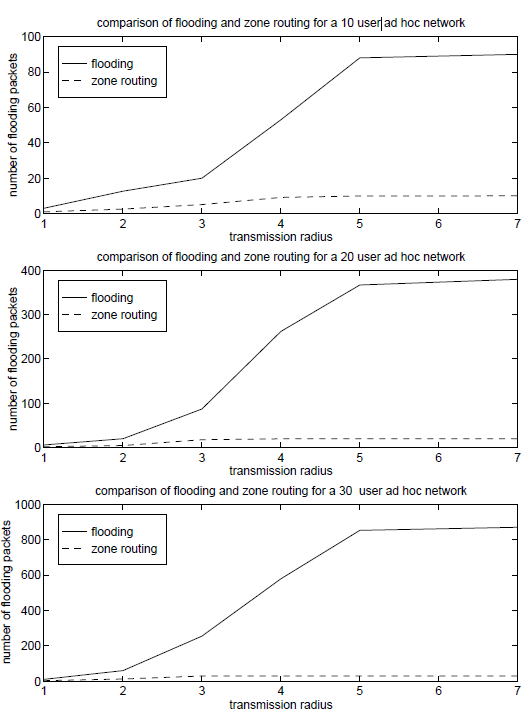
\includegraphics[width=0.5\textwidth]{ZRP.png}
    \caption{Graphs comparing number of control messages sent in ZRP vs. flooded routing \cite{haas}}
\end{figure}
Some challenges with ZRP are efficiently choosing a zone radius or handling different sized zones.
\subsection{FSR}
Fisheye State Routing is a proactive Hierarchical routing protocol. Each node keeps a routing table containing periodically updated information on the location and path to other nodes in the mesh network.  Instead of tracking all changes, FSR updates
information about nodes further away less frequently, similar to how a fish-eye lens is less detailed the further you move from the center\cite{enwiki:987177004}. Route computation is performed using Dijkstra's algorithm. Degradation of packet quality due to less frequent routing 
updates for distant nodes is not an issue because each node along the path has updated information on its neighboring nodes.  FSR was never publicly implemented as a standalone protocol, but other protocols such as OLSR and OrderOne are heavily based on
the fundamental principles of FSR. One notable drawback with FSR is that when a node disconnects, neighboring nodes update their routing tables much faster than other nodes further away, and the differences between the tables can lead to temporary loops forming.
These loops are also present in implementations of OLSR.
\subsection{OrderOne}
OrderOne is a proprietary hierarchical protocol based partially on the FSR protocol.  Nodes select a parent node from adjacent connections, choosing the direction that leads to the most other nodes. Eventually a tree is formed with a small number of root nodes.
Each node then pushes a route from that location to the roots of the tree. When a message needs to be sent, nodes can push it to the root, where a path is guaranteed to be stored in the root's routing table. OrderOne then uses Dijkstra's algorithm to optimize the pathing\cite{enwiki:618641168}.

OrderOne's protocol has a number of benefits, including the ability to support many more nodes on a single network, and the flexibility to support both low-power and high-power nodes\cite{boland_2007}. Restricting the routing table storage to the route nodes minimizes the strain on nonroot nodes.
The only limit on connectable nodes is having enough memory on the root nodes to track and update the route tables.  For larger networks, root nodes would need to be fairly high powered and well maintained.  Similar to the FSR protocol that OrderOne is built on, issues with bandwidth 
at the edges of the network are compensated for by greatly reduced traffic further from the root. As OrderOne is a proprietary protocol, licensing is required for it's use. Most of the protocols previously mentioned are already implemented into the Linux kernel.
\subsection{ZigBee}
ZigBee is a low-power, low-cost, short-range ad hoc network protocol suite for sensor networks and Internet of Things (IoT) systems.  
\begin{figure}[h]
    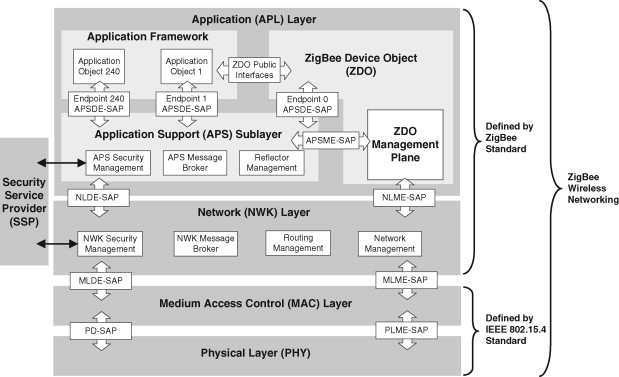
\includegraphics[width=0.5\textwidth]{zigbee.jpg}
    \caption{ZigBee protocol layers\cite{amin_saeed_2018}}
\end{figure}
ZigBee devices have a fairly limited range of up to 100 meters, but their range can be extended through an intermediate mesh network with another protocol.
ZigBee is built across several network layers, from the physical layer to the application layer. 

Tree, star and generic mesh networks are supported by the protocol, but a coordinator device is required to manage routes, while individual devices manage connections to the network\cite{enwiki:999715964}.  Special 
ZigBee routers allow for the rest of the mesh to connect to a larger network.  ZigBee is also a cryptographically secure network; most protocols are not.  
\section{Real-World Applications}
Mesh networks have a wide variety of applications in many different fields and circumstances.  Previous sections have touched on some of these applications such as military applications and IoT. Two more are covered in detail below, Portable Network kits for decentralized internet service, 
and the Iridium Constellation, a set of 66 phone and data satellites in a mesh configuration.
\subsection{Neighborhood-wide Mesh Networks}
Commotion is an open source wireless mesh network system developed by the Open Technology Institute for bringing decentralized internet and emergency response communications to neighborhoods. The system is based on the OLSR protocol\cite{enwiki:986340162}, and packs everything necessary for running a node into a solar powered suitcase called a Portable Network Kit (PNK). People connecting to 
the network also need to install the commotion firmware on their routers. The system was successfully deployed in Red Hook, Brooklyn, in 2012. After hurricane Sandy devastated New York, Red Hook was able to maintain their network using the PNKs\cite{byrum_2020}. 
\begin{figure}[h]
    \centering
    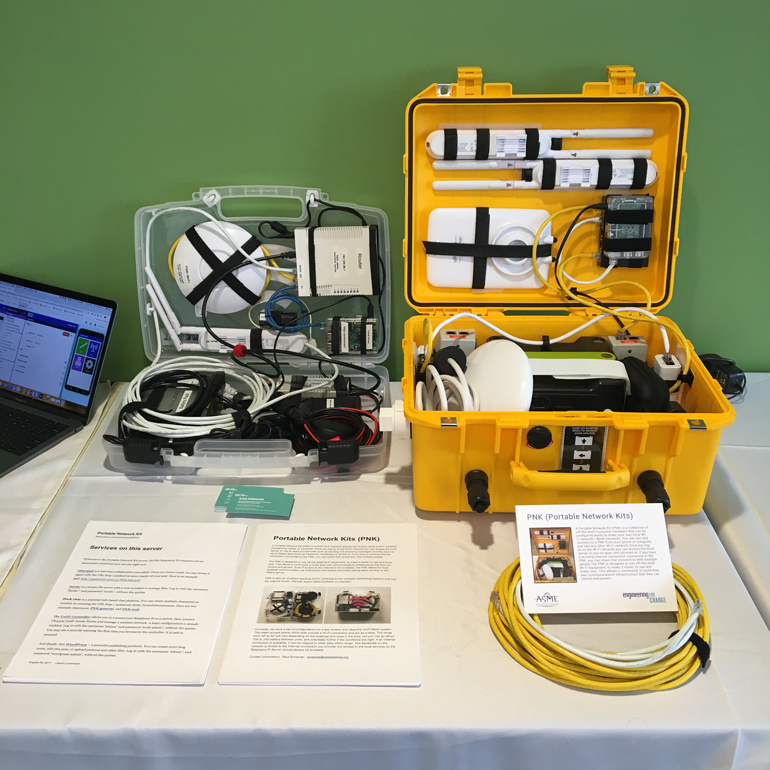
\includegraphics[width=0.35\textwidth]{pnk.jpg}
    \caption{Portable Network Kits for deploying community mesh networks}
\end{figure}
\subsection{The Iridium Constellation}
The Iridium Satellite Constellation consists of 66 low earth orbit satellites with microwave based cross-link beams allowing the satellites to communicate in a mesh type configuration.  Routing of calls is handled as part of the network, eliminating the need for multiple ground based towers. Some towers exist to help improve the network's stability. The satellites are also 
able to hand off calls to adjacent satellites as they rotate out of view of the person making the call. \cite{enwiki:1004659358}
\section{Areas for Improvement}
Wireless mesh networks have a lot of advantages over traditional wired and cellular networks, including flexibility and availability especially in remote areas.  There are some drawbacks to implementing and maintaining mesh networks, however. One is network security. Individual nodes serve as both clients and routers for the network. Limiting the ability of these nodes to disrupt service or
flood the network with packets is challenging.  ZigBee is a highly secure mesh network, but the protocols reach down into the hardware layer, and the radios are usually embedded into the device.  This level of control isn't possible on a network where any device can participate. To prevent some of the most common attacks, improving the security of the protocols on the network layer 
can have a big impact. In particular, protocols such as Wormhole detection based on neighbor's neighbor scheme (WDNN) and Position aware secure and efficient route discovery protocol for wireless mesh network (PASER) are capable of verifying the true location of nodes and encrypting the messages transmitted through them\cite{7454499}.

Another major issue is high latency in the network, especially when nodes drop out. Often it can take several seconds for a broken link to be discovered and fixed. One possible solution to this problem is to use Opportunistic routing and Network Coding to reduce lessen the time spent rerouting lost nodes\cite{8319326}. 
\newpage
By maintaining multiple paths and tracking the amount of data travelling through the nodes
at any given time, packets can be sent with minimal loss and redundancy compensates for lost connections.
\begin{figure}[h]
    \centering
    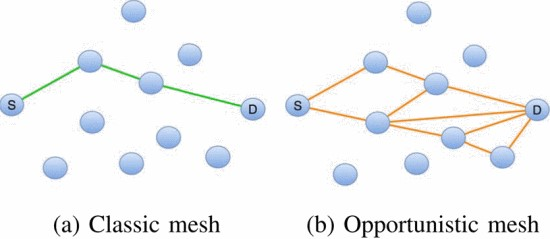
\includegraphics[width=0.45\textwidth]{opportunistic.jpg}
    \caption{Comparison of links in normal vs opportunistic mesh network}
\end{figure}
\section{Conclusion}
Wireless mesh networks offer a level of flexibility and adaptability that is hard to achieve in traditional wired systems. There are a wide variety of routing protocols with different use cases, and newer protocols with improved security and reliability are being developed. While some technological knowledge is required to set up a mesh network from scratch, plug and play networks such as Google WiFi 
and ZigBee based IoT smart home devices are bringing mesh networks into the mainstream. Overall, mesh networks are an important way to connect large numbers of devices without requiring expensive infrastructure, and offer many opportunities for more efficient communications.
\newpage
\printbibliography
\end{document}